\documentclass[11pt,a4paper]{article}
\usepackage[textwidth=37em,vmargin=30mm]{geometry}
\usepackage{calc,xunicode,amsmath,amssymb,paralist,enumitem,tabu,booktabs,datetime2,xeCJK,xeCJKfntef,listings}
\usepackage{tocloft,fancyhdr,tcolorbox,xcolor,graphicx,eso-pic,xltxtra,xelatexemoji}

\usepackage[hidelinks]{hyperref}
\hypersetup{
    colorlinks=false,
    pdfpagemode=FullScreen,
    pdftitle={Web Digest - 2023-01-10}
}

\setdefaultleftmargin{2em}{2em}{1em}{1em}{1em}{1em}

\usepackage{xeCJK,xeCJKfntef}
\newcommand{\myvphantom}[0]{\vphantom{QWERTYUIOPASDFGHJKLZXCVBNMqwertyuiopasdfghjklzxcvbnm1234567890ςρθδφγηξλζχψβμ\"A}}
\xeCJKsetup{PunctStyle=plain,RubberPunctSkip=false,CJKglue=\myvphantom\hskip 0pt plus 0.1em minus 0.05em,CJKecglue=\myvphantom\hskip 0.22em plus 200pt}
\XeTeXlinebreaklocale "zh"
\XeTeXlinebreakskip = 0pt


\setmainfont{Brygada 1918}
\setromanfont{Brygada 1918}
\setsansfont{IBM Plex Sans}
\setmonofont{JetBrains Mono NL}
\setCJKmainfont{Noto Serif CJK SC}
\setCJKromanfont{Noto Serif CJK SC}
\setCJKsansfont{Noto Sans CJK SC}
\setCJKmonofont{Noto Sans CJK SC}

\setlength{\parindent}{0pt}
\setlength{\parskip}{8pt}
\linespread{1.15}

\lstset{
	basicstyle=\ttfamily\footnotesize,
	numbersep=5pt,
	backgroundcolor=\color{black!5},
	showspaces=false,
	showstringspaces=false,
	showtabs=false,
	tabsize=2,
	captionpos=b,
	breaklines=true,
	breakatwhitespace=true,
	breakautoindent=true,
	linewidth=\textwidth
}






\newcommand{\coverpic}[2]{
    % argv: itemurl, authorname
    Cover photo by #2~~(\href{#1}{#1})
}
\newcommand{\makeheader}[0]{
    \begin{titlepage}
        % \newgeometry{hmargin=15mm,tmargin=21mm,bmargin=12mm}
        \begin{center}
            
            \rmfamily\scshape
            \fontspec{BaskervilleF}
            \fontspec{Old Standard}
            \fontsize{59pt}{70pt}\selectfont
            WEB\hfill DIGEST
            
            \vfill
            % \vskip 30pt
            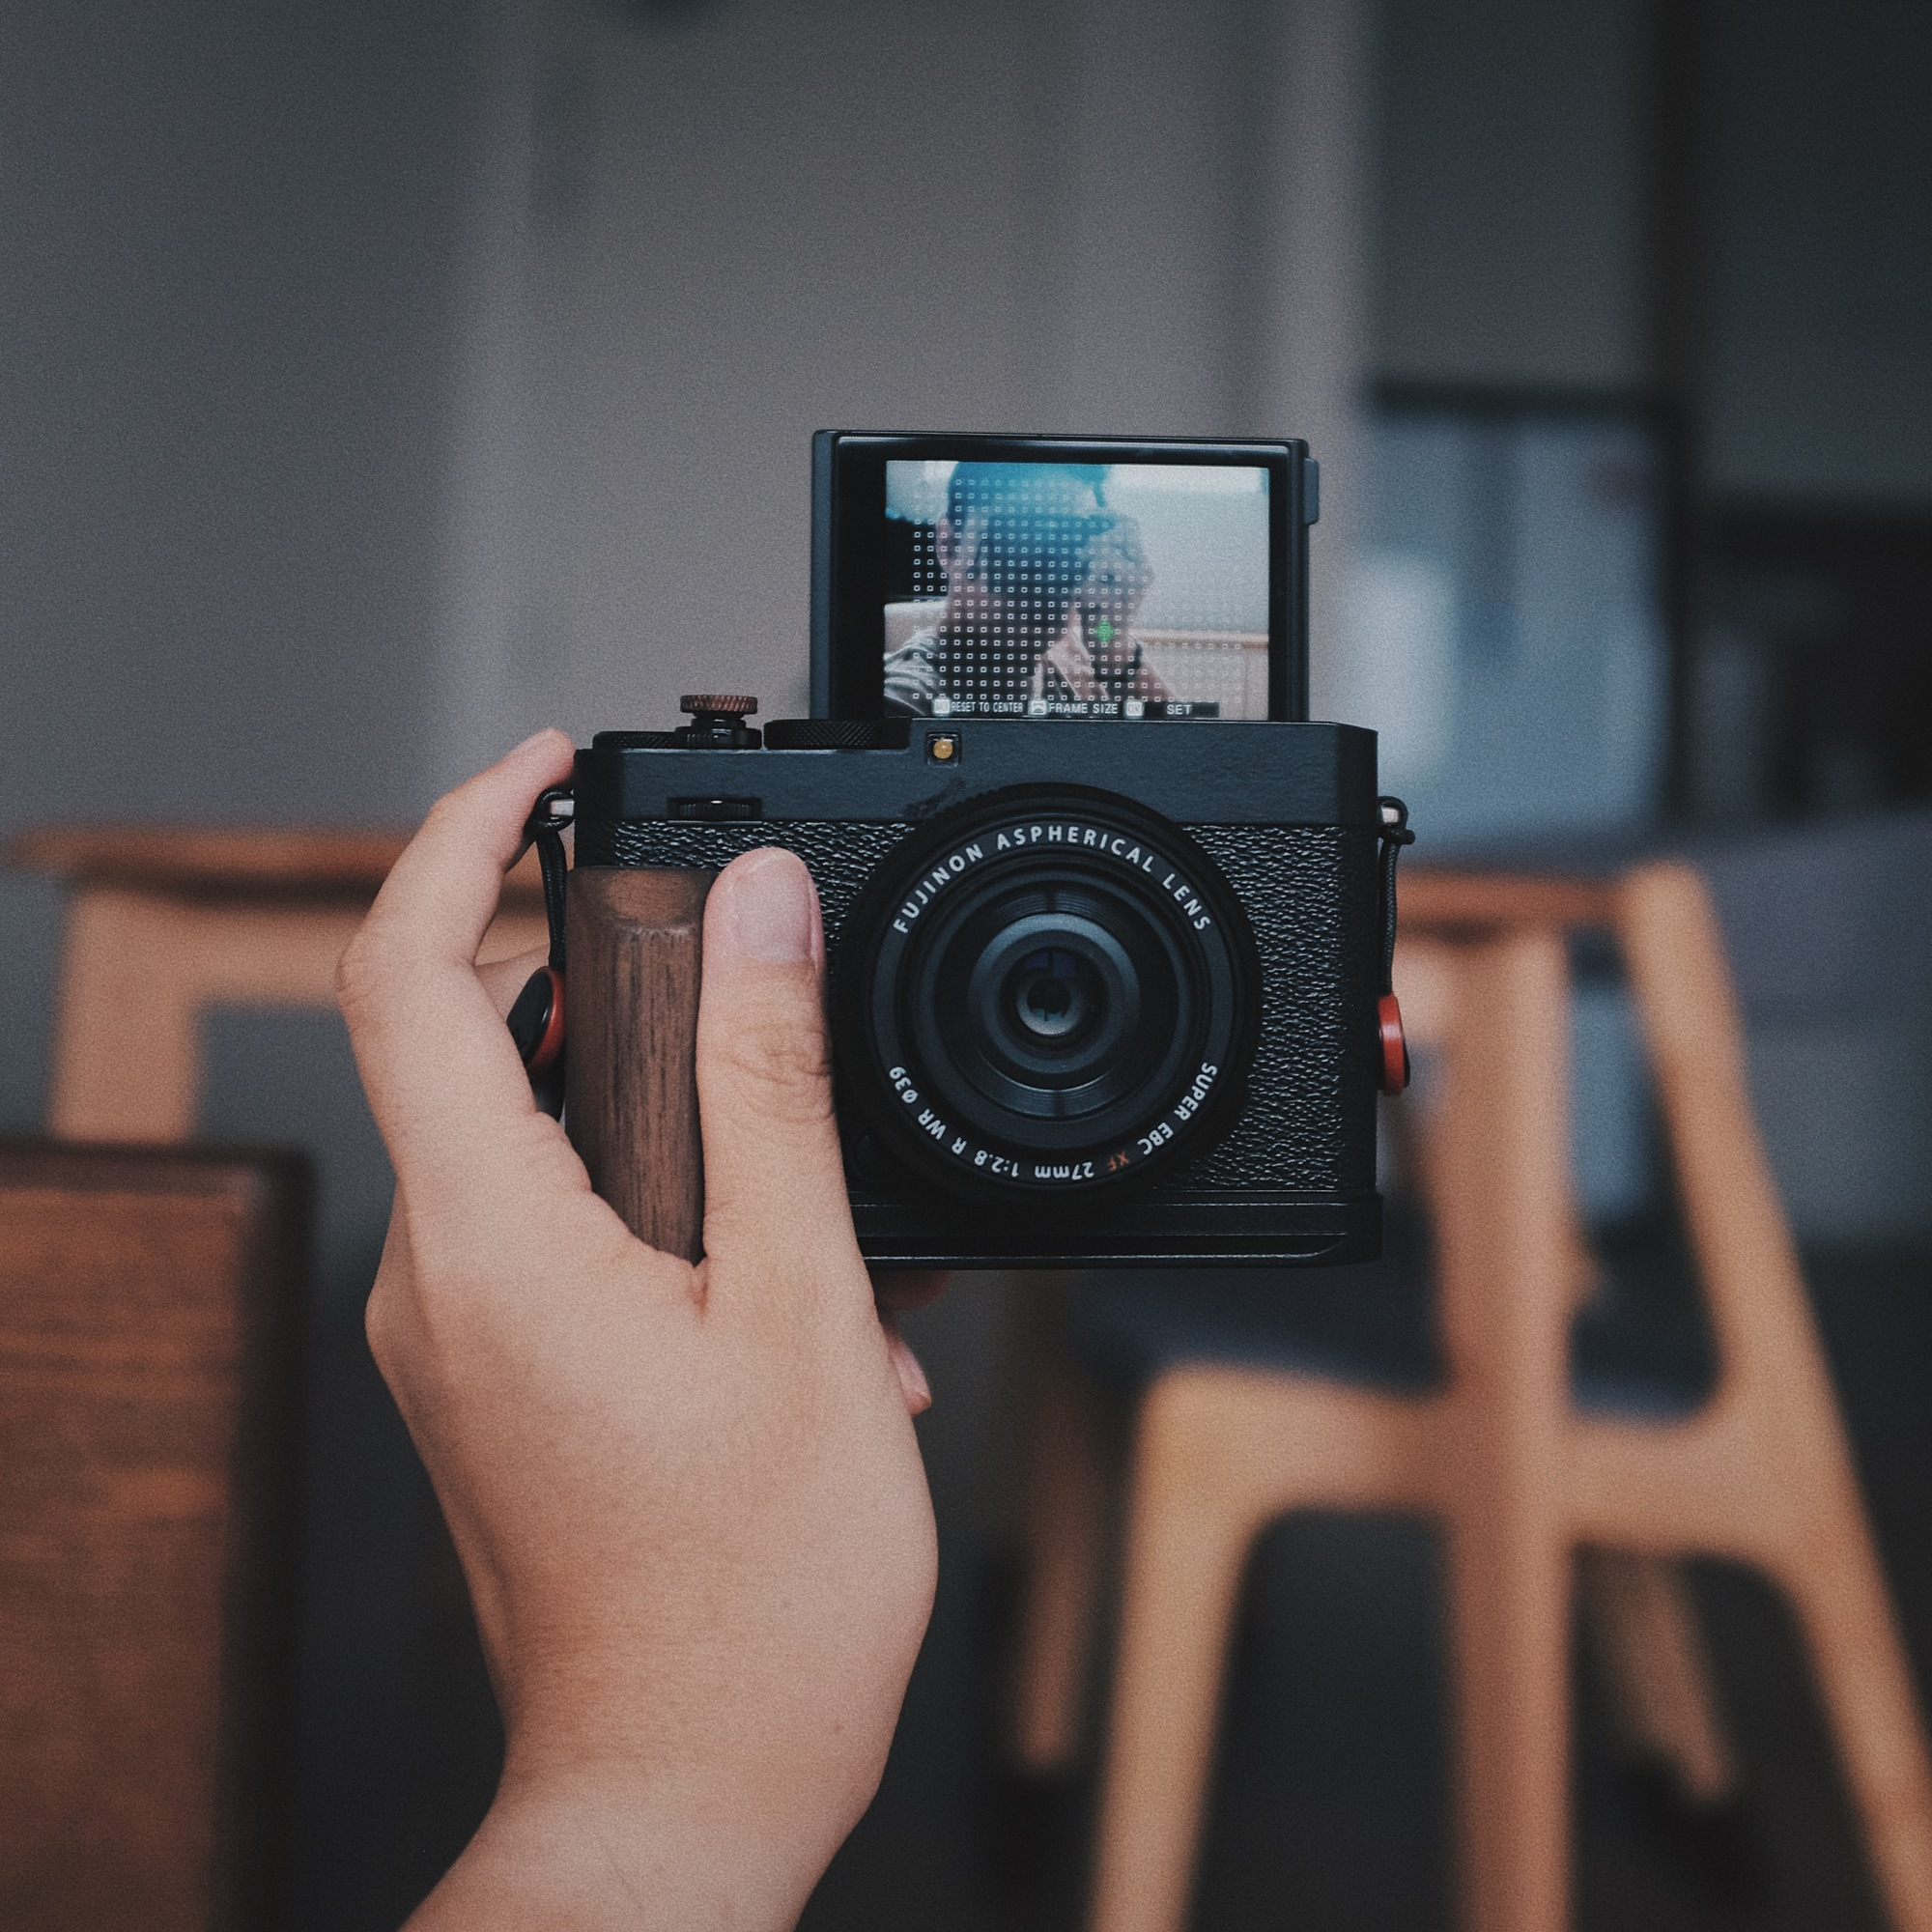
\includegraphics[width=\linewidth]{webdb/2023/20230110/final/coverpic-prod.jpg}\par
            % \vskip 30pt
            \vfill

            \normalsize\rmfamily\scshape
            \copyright{} The Web Digest Project \hfill\large 2023-01-10
        \end{center}
    \end{titlepage}
    % \restoregeometry
}
\newcommand{\simplehref}[1]{%
    \textcolor{blue!80!green}{\href{#1}{#1}}%
}
\renewcommand{\contentsname}{\center\Huge\sffamily\bfseries Contents\par\vskip 20pt}
\newcounter{ipartcounter}
\setcounter{ipartcounter}{0}
\newcommand{\ipart}[1]{
    % \vskip 20pt
    \clearpage
    \stepcounter{ipartcounter}
    \phantomsection
    \addcontentsline{toc}{section}{#1}
    \begin{center}
        \Huge
        \sffamily\bfseries
        #1
    \end{center}
    \vskip 20pt
}
\newcommand{\entrytitlefont}[0]{\Large\sffamily\bfseries}
\newcommand{\entryitemGeneric}[2]{
    % argv: title, url
    \parbox{\linewidth}{
        \entrytitlefont#1\par\vskip 5pt
        \footnotesize\ttfamily\mdseries
        \simplehref{#2}\par
    }\vskip 11pt
}
\newcommand{\entryitemGithub}[3]{
    % argv: title, url, desc
    \parbox{\linewidth}{
        \entrytitlefont#1\par\vskip 5pt
        \footnotesize\ttfamily\mdseries
        \simplehref{#2}\par\vskip 5pt
        \small\rmfamily\mdseries#3
    }\vskip 11pt
}
\newcommand{\entryitemAp}[3]{
    % argv: title, url, desc
    \parbox{\linewidth}{
        \entrytitlefont#1\par\vskip 5pt
        \footnotesize\ttfamily\mdseries
        \simplehref{#2}\par\vskip 5pt
        \small\rmfamily\mdseries#3
    }\vskip 11pt
}
\newcommand{\entryitemHackernews}[3]{
    % argv: title, hnurl, rawurl
    \parbox{\linewidth}{
        \entrytitlefont#1\par\vskip 5pt
        \footnotesize\ttfamily\mdseries
        \simplehref{#3}\par
        \textcolor{black!50}{\href{#2}{#2}}\par
    }\vskip 11pt
}






\begin{document}

\makeheader

\tableofcontents\clearpage


\ipart{Hacker News}
\entryitemTwoLinks{\hskip 0pt{}The first time I'm aware that Meta is taking back signed, FTE offers}{https://news.ycombinator.com/item?id=34316618}{https://twitter.com/gergelyorosz/status/1612565777407938560}

\entryitemTwoLinks{\hskip 0pt{}I measured the pollution from my gas stove}{https://news.ycombinator.com/item?id=34316613}{https://www.distilled.earth/p/i-measured-the-pollution-from-my}

\entryitemTwoLinks{\hskip 0pt{}Texas Records All Inmates Last Words Before Execution And Puts Them All Online}{https://news.ycombinator.com/item?id=34315969}{https://www.tdcj.texas.gov/death\_row/dr\_executed\_offenders.html}

\entryitemTwoLinks{\hskip 0pt{}Just: A Command Runner}{https://news.ycombinator.com/item?id=34315779}{https://github.com/casey/just}

\entryitemTwoLinks{\hskip 0pt{}Tomu – A family of devices which fit inside your USB port}{https://news.ycombinator.com/item?id=34315533}{https://tomu.im/}

\entryitemTwoLinks{\hskip 0pt{}A single developer dropped AWS costs by 90\%, then disappeared}{https://news.ycombinator.com/item?id=34315499}{https://medium.com/@maximetopolov/how-a-single-developer-dropped-aws-costs-by-90-then-disappeared-2b46a115103a}

\entryitemTwoLinks{\hskip 0pt{}3D in CSS}{https://news.ycombinator.com/item?id=34315380}{https://garden.bradwoods.io/notes/css/3d}

\entryitemTwoLinks{\hskip 0pt{}England just made gigabit internet a legal requirement for new homes}{https://news.ycombinator.com/item?id=34315094}{https://www.theverge.com/2023/1/9/23546401/gigabit-internet-broadband-england-new-homes-policy}

\entryitemTwoLinks{\hskip 0pt{}An Open Letter on the Open Gaming License, to Wizards of the Coast}{https://news.ycombinator.com/item?id=34314448}{https://www.opendnd.games}

\entryitemTwoLinks{\hskip 0pt{}Raspberry Pi's Camera Module 3 adds autofocus and new Sony sensor}{https://news.ycombinator.com/item?id=34314272}{https://www.jeffgeerling.com/blog/2023/raspberry-pis-camera-module-3-adds-autofocus-and-new-sony-sensor}

\entryitemTwoLinks{\hskip 0pt{}We're wasting money by only supporting gzip for raw DNA files}{https://news.ycombinator.com/item?id=34313589}{http://www.bioinformaticszen.com/post/use-zstd-for-raw-fastq/}

\entryitemTwoLinks{\hskip 0pt{}How to store your app's entire state in the url}{https://news.ycombinator.com/item?id=34312546}{https://www.scottantipa.com/store-app-state-in-urls}

\entryitemTwoLinks{\hskip 0pt{}Japan, US to step up cooperation in developing next-generation nuclear reactors}{https://news.ycombinator.com/item?id=34312338}{https://asianews.network/japan-us-to-step-up-cooperation-in-developing-next-generation-nuclear-reactors/}

\entryitemTwoLinks{\hskip 0pt{}Show HN: HyperLogLog in Zig}{https://news.ycombinator.com/item?id=34312335}{https://github.com/axiomhq/zig-hyperloglog}

\entryitemTwoLinks{\hskip 0pt{}Ask HN: What are the foundational texts for learning about AI/ML/NN?}{https://news.ycombinator.com/item?id=34312248}{https://news.ycombinator.com/item?id=34312248}

\entryitemTwoLinks{\hskip 0pt{}I went through a period where I loaned money to anyone that asked me}{https://news.ycombinator.com/item?id=34312066}{https://twitter.com/id\_aa\_carmack/status/1612484342567010306}

\entryitemTwoLinks{\hskip 0pt{}Fake it until you automate it}{https://news.ycombinator.com/item?id=34311192}{https://understandlegacycode.com/blog/fake-it-until-you-automate-it/}

\entryitemTwoLinks{\hskip 0pt{}Mind Your Own Business Act of 2021}{https://news.ycombinator.com/item?id=34311048}{https://www.congress.gov/bill/117th-congress/senate-bill/1444}

\entryitemTwoLinks{\hskip 0pt{}Sourcehut will blacklist the Go module mirror}{https://news.ycombinator.com/item?id=34310674}{https://sourcehut.org/blog/2023-01-09-gomodulemirror/}

\entryitemTwoLinks{\hskip 0pt{}'Terminator' 1 and 2 Save Their Reveals for the Right Time}{https://news.ycombinator.com/item?id=34310607}{https://textualvariations.substack.com/p/terminator-thoughts}


\ipart{V2EX}
\entryitemGeneric{\hskip 0pt{}[分享发现] 《东北之夏》已上架 Steam!}{https://www.v2ex.com/t/907774}

\entryitemGeneric{\hskip 0pt{}[分享发现] H2O - an optimized HTTP server}{https://www.v2ex.com/t/907773}

\entryitemGeneric{\hskip 0pt{}[酷工作] [上海]-[不加班]-[外企] 招 中级前端(重 Vue)和.Net(3 年起, 15-23K),高级 Java (25-35K)}{https://www.v2ex.com/t/907772}

\entryitemGeneric{\hskip 0pt{}[问与答] 14pm 信号满格 5g 在线无法上网,你们遇过到吗?}{https://www.v2ex.com/t/907771}

\entryitemGeneric{\hskip 0pt{}[Apple] 京东自营 ULT-unite 雷电 4 线材这么便宜,是有什么坑吗?还是价格回归价值?}{https://www.v2ex.com/t/907770}

\entryitemGeneric{\hskip 0pt{}[分享发现] How I program C by Eskil Steenberg}{https://www.v2ex.com/t/907769}

\entryitemGeneric{\hskip 0pt{}[问与答] 你多久没发呆了?}{https://www.v2ex.com/t/907767}

\entryitemGeneric{\hskip 0pt{}[程序员] JavaScript with 为什么不推荐使用,其它语言如 Kotlin with 不是用得正酣吗}{https://www.v2ex.com/t/907766}

\entryitemGeneric{\hskip 0pt{}[macOS] MBP 的音频输出有时候会自己切到左声道}{https://www.v2ex.com/t/907765}

\entryitemGeneric{\hskip 0pt{}[宽带症候群] SFTP 传文件(不过墙)上下行都只能跑到带宽十分之一,怎么排查哪里的问题?好几个月了,一点相关资料都找不到。FTP(S)要开多个端口。除了这 3 个似乎没有别的稍微主流一点的原生支持上传的断点续传的协议了}{https://www.v2ex.com/t/907763}

\entryitemGeneric{\hskip 0pt{}[全球工单系统] 微博 - 注册 - 手机格式错误}{https://www.v2ex.com/t/907762}

\entryitemGeneric{\hskip 0pt{}[程序员] 新手最近在学习 Go,学习的时候有个小问题这几天我一直觉得很困扰。。求助一下大佬们}{https://www.v2ex.com/t/907760}

\entryitemGeneric{\hskip 0pt{}[旅行] [过年顺风车] 武汉到商城}{https://www.v2ex.com/t/907759}

\entryitemGeneric{\hskip 0pt{}[分享发现] TIKTOK 前端工程师恐怖如斯}{https://www.v2ex.com/t/907756}

\entryitemGeneric{\hskip 0pt{}[macOS] 有什么安卓模拟器可以跑在 arm 的 mac 上吗}{https://www.v2ex.com/t/907755}

\entryitemGeneric{\hskip 0pt{}[问与答] iOS Safari 无痕模式使用谷歌搜索 bug}{https://www.v2ex.com/t/907754}

\entryitemGeneric{\hskip 0pt{}[Apple] Safari 的扩展能读写书签吗?}{https://www.v2ex.com/t/907753}

\entryitemGeneric{\hskip 0pt{}[分享创造] 想要出海的独立开发者们,我创建了一个 subreddit,欢迎加入 pitch 你的作品!}{https://www.v2ex.com/t/907752}

\entryitemGeneric{\hskip 0pt{}[问与答] 请问有人知道现在 QQ 微信的审核机器人逻辑吗?}{https://www.v2ex.com/t/907750}

\entryitemGeneric{\hskip 0pt{}[分享创造] TeraBox- 国内资本家的国外网盘,容量 1T}{https://www.v2ex.com/t/907749}

\entryitemGeneric{\hskip 0pt{}[问与答] 求推荐电视机盒子,家里老人用}{https://www.v2ex.com/t/907748}

\entryitemGeneric{\hskip 0pt{}[问与答] 朋友们,有什么好办法测试程序在大端情况下能跑吗?}{https://www.v2ex.com/t/907747}

\entryitemGeneric{\hskip 0pt{}[macOS] Mac OS 的系统图标怎么更换样式?}{https://www.v2ex.com/t/907746}

\entryitemGeneric{\hskip 0pt{}[问与答] 2023 年了, 16 寸 Windows 轻薄办公本求推荐, 6K+}{https://www.v2ex.com/t/907745}

\entryitemGeneric{\hskip 0pt{}[酷工作] [上海]-[不加班]-[外企] 招 中级前端(重 Vue)和.Net(3 年起, 15-23K),高级 Java (25-35K)}{https://www.v2ex.com/t/907744}

\entryitemGeneric{\hskip 0pt{}[Java] Java 导出 word 解决方案}{https://www.v2ex.com/t/907743}

\entryitemGeneric{\hskip 0pt{}[程序员] CI CD -> Git 分支管理}{https://www.v2ex.com/t/907742}

\entryitemGeneric{\hskip 0pt{}[程序员] Java 和 Python 抉择}{https://www.v2ex.com/t/907740}

\entryitemGeneric{\hskip 0pt{}[程序员] Alan 的 Docker 容器学习笔记}{https://www.v2ex.com/t/907739}

\entryitemGeneric{\hskip 0pt{}[问与答] 毕业了有点迷茫..求赐教}{https://www.v2ex.com/t/907738}

\entryitemGeneric{\hskip 0pt{}[酷工作] 招聘远程岗位——前端开发工程师、UI 设计师}{https://www.v2ex.com/t/907736}

\entryitemGeneric{\hskip 0pt{}[问与答] 求助,修改 微信一键登录 的账号名称和头像}{https://www.v2ex.com/t/907735}

\entryitemGeneric{\hskip 0pt{}[问与答] 为啥 win10 和 win11 的任务管理器都会卡住?是普遍 Bug?}{https://www.v2ex.com/t/907734}

\entryitemGeneric{\hskip 0pt{}[酷工作] [web3 职位] [知名 NFT 数据平台] 后端负责人/前端负责人}{https://www.v2ex.com/t/907733}

\entryitemGeneric{\hskip 0pt{}[分享发现] 分享一些遇到的非常有趣的网站}{https://www.v2ex.com/t/907732}

\entryitemGeneric{\hskip 0pt{}[北京] 请教,空档期如何自缴社保?}{https://www.v2ex.com/t/907731}

\entryitemGeneric{\hskip 0pt{}[问与答] 关于背调,离职理由需要一致吗?}{https://www.v2ex.com/t/907726}

\entryitemGeneric{\hskip 0pt{}[宽带症候群] 广西联通动手了,普通家宽和公网 IP 说拜拜。}{https://www.v2ex.com/t/907724}

\entryitemGeneric{\hskip 0pt{}[问与答] 软路由 R2S 无法上网}{https://www.v2ex.com/t/907723}

\entryitemGeneric{\hskip 0pt{}[问与答] 修改小区物业前期合同问题,怎么 pk 物业,业委会有必要吗}{https://www.v2ex.com/t/907721}

\entryitemGeneric{\hskip 0pt{}[程序员] GitKarken 破解版}{https://www.v2ex.com/t/907720}

\entryitemGeneric{\hskip 0pt{}[问与答] Tesla 车友们,你们车险多少一年}{https://www.v2ex.com/t/907719}

\entryitemGeneric{\hskip 0pt{}[问与答] 想不明白:大学生想买 iPhone14 奈何没钱 使用白条 和 找朋友借钱买手机}{https://www.v2ex.com/t/907717}

\entryitemGeneric{\hskip 0pt{}[宽带症候群] 神奇的广电宽带,没有 vlan 怎么破}{https://www.v2ex.com/t/907715}

\entryitemGeneric{\hskip 0pt{}[macOS] 无边记存储几张截图很卡,内存占用也很大}{https://www.v2ex.com/t/907713}

\entryitemGeneric{\hskip 0pt{}[问与答] Chromecast 是不是旅行中接酒店电视看流媒体的神器?}{https://www.v2ex.com/t/907711}

\entryitemGeneric{\hskip 0pt{}[Apple] 想了解一下大家在 ios 上下载网页视频/音频和播放的 app 或者办法}{https://www.v2ex.com/t/907710}

\entryitemGeneric{\hskip 0pt{}[酷工作] 坐标上海静安寺周边,小而美北欧游戏公司资深客户端开发,资深服务端开发岗位分享 ing}{https://www.v2ex.com/t/907709}

\entryitemGeneric{\hskip 0pt{}[问与答] 币安有人玩么?}{https://www.v2ex.com/t/907708}

\entryitemGeneric{\hskip 0pt{}[职场话题] 公司以受疫情影响为由,强制降薪,如何主张赔偿}{https://www.v2ex.com/t/907707}

\ipart{Solidot}
\entryitemGeneric{\hskip 0pt{}Debian 移除 Python 2}{https://www.solidot.org/story?sid=73791}

\entryitemGeneric{\hskip 0pt{}DistroWatch 的二十年}{https://www.solidot.org/story?sid=73790}

\entryitemGeneric{\hskip 0pt{}Linux Mint 21.1 释出}{https://www.solidot.org/story?sid=73717}

\entryitemGeneric{\hskip 0pt{}Linux 内核贡献成熟度模型}{https://www.solidot.org/story?sid=73677}

\entryitemGeneric{\hskip 0pt{}内核补丁将 kallsyms\_lookup\_name()查找速度提高 715 倍}{https://www.solidot.org/story?sid=73648}

\entryitemGeneric{\hskip 0pt{}Linux 6.1 释出}{https://www.solidot.org/story?sid=73621}

\entryitemGeneric{\hskip 0pt{}费米实验室和 CERN 选择 AlmaLinux}{https://www.solidot.org/story?sid=73595}

\entryitemGeneric{\hskip 0pt{}Steam Linux 市场份额达到 1.44\%}{https://www.solidot.org/story?sid=73543}

\entryitemGeneric{\hskip 0pt{}微软称 WSL 达到了 GA 阶段}{https://www.solidot.org/story?sid=73451}

\entryitemGeneric{\hskip 0pt{}Fedora 37 发布}{https://www.solidot.org/story?sid=73387}

\entryitemGeneric{\hskip 0pt{}开源 Linux 平板电脑,预装 FydeOS 出货}{https://www.solidot.org/story?sid=73256}

\entryitemGeneric{\hskip 0pt{}钓鱼网站在 Google 上伪装成 GIMP 打广告}{https://www.solidot.org/story?sid=73245}

\entryitemGeneric{\hskip 0pt{}Fedora Linux 37 为修复高危漏洞推迟发布}{https://www.solidot.org/story?sid=73198}

\entryitemGeneric{\hskip 0pt{}Rust for Linux 项目下一步发展计划}{https://www.solidot.org/story?sid=73165}

\entryitemGeneric{\hskip 0pt{}Linux 考虑淘汰对英特尔 i486 CPU 的支持}{https://www.solidot.org/story?sid=73155}

\entryitemGeneric{\hskip 0pt{}Ubuntu 22.10 Kinetic Kudu 发布}{https://www.solidot.org/story?sid=73140}

\entryitemGeneric{\hskip 0pt{}Tails 5.5 发布}{https://www.solidot.org/story?sid=73107}

\entryitemGeneric{\hskip 0pt{}Ubuntu 终端广告惹恼用户}{https://www.solidot.org/story?sid=73098}

\entryitemGeneric{\hskip 0pt{}Linus Torvalds 呼吁内核开发者不要在截止日期前递交补丁}{https://www.solidot.org/story?sid=73088}

\entryitemGeneric{\hskip 0pt{}Linux 6.1-rc1 释出}{https://www.solidot.org/story?sid=73081}

\ipart{联合早报}
\entryitemGeneric{\hskip 0pt{}解放军两周来二度于台海周边大型军演 学者:大陆军机演习频率料再创新高}{https://www.zaobao.com/news/china/story20230110-1351792}

\entryitemGeneric{\hskip 0pt{}要与美等民主阵营一起发展经济 赖清德吁勿让``疑美论''成为台湾社会共识}{https://www.zaobao.com/news/china/story20230110-1351793}

\entryitemGeneric{\hskip 0pt{}德国会代表团访台北京表不满 中国驻德大使指德对华新战略 以意识形态为主导不利合作}{https://www.zaobao.com/news/china/story20230110-1351794}

\entryitemGeneric{\hskip 0pt{}紫禁城故宫邮局开业}{https://www.zaobao.com/news/china/story20230110-1351795}

\entryitemGeneric{\hskip 0pt{}刚出任市委副书记 陈之常任命为南京代理市长}{https://www.zaobao.com/news/china/story20230110-1351796}

\entryitemGeneric{\hskip 0pt{}巴拉圭众议院议长访台 蔡英文吁共同捍卫民主}{https://www.zaobao.com/news/china/story20230110-1351797}

\entryitemGeneric{\hskip 0pt{}早说}{https://www.zaobao.com/news/china/story20230110-1351798}

\entryitemGeneric{\hskip 0pt{}赴港大陆游客为何不如预期多?}{https://www.zaobao.com/news/china/story20230110-1351799}

\entryitemGeneric{\hskip 0pt{}中国重开边境 民众抢办护照签证}{https://www.zaobao.com/news/china/story20230110-1351801}

\entryitemGeneric{\hskip 0pt{}中国医保局: 与辉瑞谈判不成功 Paxlovid太贵不纳入医保}{https://www.zaobao.com/news/china/story20230110-1351802}

\entryitemGeneric{\hskip 0pt{}张文宏:中国有能力把冠病转为地方性流行病}{https://www.zaobao.com/news/china/story20230110-1351803}

\entryitemGeneric{\hskip 0pt{}``动态清零''走入历史 中国敞开国门 拥抱疫后世界}{https://www.zaobao.com/news/china/story20230109-1351414}

\entryitemGeneric{\hskip 0pt{}恢复免检疫通关 北上港人远超南下陆客}{https://www.zaobao.com/news/china/story20230109-1351415}

\entryitemGeneric{\hskip 0pt{}侧记:久别重逢的笑声和泪水}{https://www.zaobao.com/news/china/story20230109-1351416}

\entryitemGeneric{\hskip 0pt{}台北市第三选区立委补选 国民党王鸿薇小胜民进党吴怡农}{https://www.zaobao.com/news/china/story20230109-1351417}

\entryitemGeneric{\hskip 0pt{}港劳工及褔利局长孙玉菡:新港各有优势和互补空间 可合作提高亚洲吸引力}{https://www.zaobao.com/news/china/story20230109-1351418}

\entryitemGeneric{\hskip 0pt{}重庆核酸检测企业大规模裁员 员工抗议并与警员冲突}{https://www.zaobao.com/news/china/story20230109-1351419}

\entryitemGeneric{\hskip 0pt{}港媒:司法部长唐一军 料出任江西省政协主席}{https://www.zaobao.com/news/china/story20230109-1351421}

\entryitemGeneric{\hskip 0pt{}早 说}{https://www.zaobao.com/news/china/story20230109-1351422}

\entryitemGeneric{\hskip 0pt{}于泽远:高官腐败令人触目惊心}{https://www.zaobao.com/news/china/story20230109-1351423}

\entryitemGeneric{\hskip 0pt{}分析:两岸论述只有目标没有方案 赖清德``和平保台''恐保不了民进党}{https://www.zaobao.com/news/china/story20230109-1351424}

\entryitemGeneric{\hskip 0pt{}江西货车雾中冲撞出殡队伍 19人死20伤}{https://www.zaobao.com/news/china/story20230109-1351425}

\ipart{AP News}
\entryitemWithDescription{\hskip 0pt{}Brazil and Jan. 6 in US: Parallel attacks, but not identical}{https://apnews.com/article/22a083f0d08bb9d1d93b67871a103b0c}{FILE - Protesters, supporters of Brazil\textquotesingle s former President Jair Bolsonaro, stand on the roof of the National Congress building after they stormed it, in Brasilia, Brazil, Sunday, Jan. 8, 2023. (AP Photo/Eraldo Peres, File...}

\entryitemWithDescription{\hskip 0pt{}DOJ reviewing potentially classified docs at Biden center}{https://apnews.com/article/812ef44a5333f6d93423a67a683fa024}{FILE - President Joe Biden waves before boarding Air Force One at El Paso International Airport in El Paso, Texas, Sunday, Jan. 8, 2023, to travel to Mexico City, Mexico. The Justice Department is reviewing a batch of potentially...}

\entryitemWithDescription{\hskip 0pt{}Having elected House speaker, Republicans try governing}{https://apnews.com/article/b9fcfd11427a695fe2eb49e36988f1a0}{Speaker of the House Kevin McCarthy, R-Calif., talks to reporters as he walks to the speaker\textquotesingle s ceremonial office at the Capitol in Washington, Monday, Jan. 9, 2023. (AP Photo/Jose Luis Magana) WASHINGTON (AP) --- Electing...}

\entryitemWithDescription{\hskip 0pt{}How Republicans are transforming the House in the majority}{https://apnews.com/article/60b4f098523b982b549823f4b3e8f9e4}{Newly-elected Speaker of the House Kevin McCarthy, R-Calif., walks to his office from the chamber after a contentious battle to lead the GOP majority in the 118th Congress, at the Capitol in Washington, Saturday, Jan. 7, 2023. (AP Photo/...}

\entryitemWithDescription{\hskip 0pt{}\$1.1B Mega Millions prize also can be winner for retailers}{https://apnews.com/article/cf5a7fc41ee94466bbe5894e1ec48615}{FILE - Mega Millions lottery tickets and a wager slip are displayed, Friday, Jan. 6, 2023, in Derry, N.H. An estimated \$1.1 billion Mega Millions jackpot drawing Tuesday, Jan. 10, 2023, has people lined up at convenience stores...}

\entryitemWithDescription{\hskip 0pt{}Bills safety Hamlin back in Buffalo to continue recovery}{https://apnews.com/article/35005f5e4ac87eca56e7d99d49eaec65}{FILE - Buffalo Bills defensive back Damar Hamlin (3) leaves the field after an NFL football game against the New England Patriots, Thursday, Dec. 1, 2022, in Foxborough, Mass. Quick on-the-field emergency care from well-rehearsed medical...}

\entryitemWithDescription{\hskip 0pt{}As Brazil reels from riots, Bolsonaro finds home in Florida}{https://apnews.com/article/099db80c6511119b534ca17747f871fe}{Former Brazil President Jair Bolsonaro, center, meets with supporters outside a vacation home where he is staying near Orlando, Fla., on Wednesday, Jan. 4, 2023. (Skyler Swisher/Orlando Sentinel via AP) KISSIMMEE, Fla. (AP) --- As Brazil...}

\entryitemWithDescription{\hskip 0pt{}Israel's Netanyahu races ahead with hard-line agenda}{https://apnews.com/article/c3419b07e43f853e9a8d44d55fc4a886}{Israeli Prime Minister Benjamin Netanyahu convenes a weekly cabinet meeting at the Prime Minister\textquotesingle s office in Jerusalem, Sunday, Jan. 8, 2023. (Ronen Zvulun/Pool Photo via AP) Prime Minister Benjamin Netanyahu's new...}

\entryitemWithDescription{\hskip 0pt{}Chief: 6-year-old shot Virginia teacher during class lesson}{https://apnews.com/article/25cebfde17e46abc435c205210a7073d}{Messages of support for teacher Abby Zwerner, who was shot by a 6 year old student, grace the front door of Richneck Elementary School Newport News, Va. on Monday Jan. 9, 2023. The Virginia teacher who authorities say was shot by a 6-year...}

\entryitemWithDescription{\hskip 0pt{}Everyone in California's Montecito ordered out amid deluge}{https://apnews.com/article/7c151eeaf3f567a125d74245173327f1}{A man wades through a flooded street in the Rio Del Mar neighborhood of Aptos, Calif., Monday, Jan. 9, 2023. (AP Photo/Nic Coury) LOS ANGELES (AP) --- Rain-weary Californians grappled with flooding and mudslides Monday as the latest in a...}

\entryitemWithDescription{\hskip 0pt{}Famed Danish restaurant Noma to start new 'flavor search'}{https://apnews.com/article/4a772a42e11833976b49be943e50bf57}{FILE -- Danish restaurant Noma in Copenhagen, March 14, 2012. The innovative Danish restaurant Noma which has reclaimed the title of world's top restaurant several times, said Monday, Jan. 9, 2023, that it will shut down and become ``a...}

\entryitemWithDescription{\hskip 0pt{}Border pressures migrate north as Venezuelans head to Denver}{https://apnews.com/article/103c21b26482306a25e08416295f9e78}{A migrant looks through donated clothes at a makeshift shelter in Denver, Friday, Jan. 6, 2023. Over the past month, nearly 4,000 immigrants, almost all Venezuelans, have arrived unannounced in the frigid city, with nowhere to stay and...}

\entryitemWithDescription{\hskip 0pt{}Georgia grand jury ends probe of Trump, 2020 election}{https://apnews.com/article/fc08d39209ce3be768d933f96a434abf}{FILE - Former President Donald Trump speaks as he announces a third run for president, at Mar-a-Lago in Palm Beach, Fla., Nov. 15, 2022. The special grand jury investigating whether then-President Donald Trump and his allies committed any...}

\entryitemWithDescription{\hskip 0pt{}UN says ozone layer slowly healing, hole to mend by 2066}{https://apnews.com/article/83794d6e5ae6c4469b60effb185d1509}{FILE - In this NASA false-color image, the blue and purple shows the hole in Earth\textquotesingle s protective ozone layer over Antarctica on Oct. 5, 2022. Earth's protective ozone layer is slowly but noticeably healing at a pace that...}

\entryitemWithDescription{\hskip 0pt{}Shiffrin can break Vonn's record -- if she can stay awake}{https://apnews.com/article/eb3b1478862676e3a3e141de7c4e2de7}{United States\textquotesingle{} Mikaela Shiffrin smiles after winning an alpine ski, women\textquotesingle s World Cup giant slalom race, in Kranjska Gora, Slovenia, Sunday, Jan. 8, 2023. Shiffrin matched Lindsey Vonn\textquotesingle s...}

\entryitemWithDescription{\hskip 0pt{}Ukraine school rejects Russian claim of troops killed there}{https://apnews.com/article/79b6b7c903985358517088278d81cebe}{Municipal workers clear the rubble on the roof of College No. 47 which was damaged by a Russian rocket attack in Kramatorsk, Ukraine, Monday, Jan. 9, 2023. (AP Photo/Evgeniy Maloletka) KRAMATORSK, Ukraine (AP) --- Officials at a...}

\entryitemWithDescription{\hskip 0pt{}Prince Harry accuses Camilla of 'dangerous' leaks to media}{https://apnews.com/article/4141be64bcd1521d1d5cf0f9b65e20b5}{A poster advertises the midnight opening of a store to sell the new book by Prince Harry called \textquotesingle Spare\textquotesingle{} in London, Monday, Jan. 9, 2023. Prince Harry has defended his memoir that lays bare rifts inside...}

\entryitemWithDescription{\hskip 0pt{}Analysis: Teammates gave Damar Hamlin the ultimate tribute}{https://apnews.com/article/2850fdfa5fd44dea388a09caa31430ba}{A video board at Levi\textquotesingle s Stadium shows a message for Damar Hamlin during an NFL football game between the San Francisco 49ers and the Arizona Cardinals in Santa Clara, Calif., Sunday, Jan. 8, 2023. (AP Photo/Jed Jacobsohn...}

\entryitemWithDescription{\hskip 0pt{}Mexico may accept more migrants expelled by US}{https://apnews.com/article/871328ff21fc6a87b698742f6e9ed3d4}{U.S. President Joe Biden is greeted at his arrival by Mexican President Andres Manuel Lopez Obrador, second left, Mexican Foreign Minister Marcelo Ebrard, second right, and U.S. Ambassador to Mexico Ken Salazar, right, at Biden...}

\entryitemWithDescription{\hskip 0pt{}CES 2023: Companies tout environmental tech innovations}{https://apnews.com/article/31d2663e9e47b6e18f99d87afc311338}{People look at a John Deere electric excavator at the John Deere booth during the CES tech show Friday, Jan. 6, 2023, in Las Vegas. (AP Photo/John Locher) LAS VEGAS (AP) --- The mottled bright green leaves of a pothos plant stood out...}

\entryitemWithDescription{\hskip 0pt{}Nurses go on strike at 2 big New York City hospitals}{https://apnews.com/article/d81f32cb7ac709404eb795a6d8822b34}{Nurses stage a strike in front of Mt. Sinai Hospital in the Manhattan borough of New York Monday, Jan. 9, 2023, after negotiations broke down hours earlier. (AP Photo/Craig Ruttle) Thousands of nurses are on strike at two major New York...}

\entryitemWithDescription{\hskip 0pt{}Cargo ship goes aground, is refloated in Egypt's Suez Canal}{https://apnews.com/article/fc27fee20b14d4017cfdc1bd7b2ffbc9}{In this photo released by Suez Canal Authority, tugboats pull the ship MV Glory in the Suez Canal between the cities of Port Said and Ismailiya, Egypt Monday, Jan. 9, 2023. A cargo ship carrying corn that went aground early on Monday in...}

\entryitemWithDescription{\hskip 0pt{}Stocks end up mixed on Wall Street after early gains fade}{https://apnews.com/article/adddcec61c0b2b377a9a38ccb10d0783}{FILE - Traders work on the floor at the New York Stock Exchange in New York, Tuesday, Oct. 4, 2022. (AP Photo/Seth Wenig, File) NEW YORK (AP) --- U.S. stocks were mixed Monday at the start of a week with a few events that could shake...}

\entryitemWithDescription{\hskip 0pt{}Kemp done being underestimated, aims to steer GOP past Trump}{https://apnews.com/article/65049bc27c3c2f5e197feaf15d1f031a}{FILE - Georgia Gov. Brian Kemp speaks at The Neighborhood Lot on July 29, 2022, in McDonough, Ga. Having vanquished both a Donald Trump-backed Republican challenger and Democratic star Stacey Abrams to win reelection, Kemp is looking to...}

\entryitemWithDescription{\hskip 0pt{}Authorities probe who was behind uprising in Brazil capital}{https://apnews.com/article/8766c0ad2fcc4ae7c8bf1aa7f9aaa0ec}{Police officers take position as supporters of Brazil\textquotesingle s former President Jair Bolsonaro leave a camp outside the Army headquarters in Brasilia, Brazil, Monday, Jan. 9, 2023. Since Bolsonaro lost re-election to Luiz Inácio...}

\entryitemWithDescription{\hskip 0pt{}New guidance: Use drugs, surgery early for obesity in kids}{https://apnews.com/article/c48d5896114beea7eda31d7b8b25461d}{This image provided by Novo Nordisk in January 2023, shows packaging for the company\textquotesingle s Wegovy drug. Children struggling with obesity should be evaluated and treated early and aggressively, with medications for kids as...}

\entryitemWithDescription{\hskip 0pt{}Hurts returns from injury, leads Eagles to No. 1 seed in NFC}{https://apnews.com/article/a80233e214f9e1b60db676bd2e5b6342}{Philadelphia Eagles quarterback Jalen Hurts throws a pass against the New York Giants during the first half of an NFL football game, Sunday, Jan. 8, 2023, in Philadelphia. (AP Photo/Matt Rourke) PHILADELPHIA (AP) --- Jalen Hurts walked...}

\entryitemWithDescription{\hskip 0pt{}Bills win for Hamlin and eliminate Patriots from playoffs}{https://apnews.com/article/25243cdf2ceb3780419859fc39537ef4}{Buffalo Bills wide receiver John Brown (16) celebrates his touchdown during the second half of an NFL football game against the New England Patriots, Sunday, Jan. 8, 2023, in Orchard Park. (AP Photo/Adrian Kraus) ORCHARD PARK, N.Y...}

\entryitemWithDescription{\hskip 0pt{}McCarthy's next big task: Win GOP support for House rules}{https://apnews.com/article/4922d22689eb79d5d05c1b49ca733123}{Dean of the House Rep. Hal Rogers, R-Ky., swears in Rep. Kevin McCarthy, R-Calif., as House Speaker on the House floor at the U.S. Capitol in Washington, early Saturday, Jan. 7, 2023. (AP Photo/Andrew Harnik) WASHINGTON (AP) --- After an...}

\entryitemWithDescription{\hskip 0pt{}Teacher shot by 6-year-old known as devoted to students}{https://apnews.com/article/2db4662a6d9f711c5bcd27b6142570a8}{Police respond to a shooting at Richneck Elementary School, Friday, Jan. 6, 2023 in Newport News, Va. A shooting at a Virginia elementary school sent a teacher to the hospital and ended with ``an individual'' in custody Friday, police and...}

\entryitemWithDescription{\hskip 0pt{}Adam Rich, former 'Eight Is Enough' child star, dies at 54}{https://apnews.com/article/7294e6bf8061f6c12604c2716d34b722}{FILE - One-time child actor Adam Rich, who starred in the 1970s TV show "Eight is Enough," walks out of a sheriff\textquotesingle s station after posting bail in City of Industry, Calif., Dec. 18, 2002. Rich, the child actor with a...}

\entryitemWithDescription{\hskip 0pt{}Pro-Bolsonaro rioters storm Brazil's top government offices}{https://apnews.com/article/0c03c098a5e2a09ac534412c30ae8355}{Protesters, supporters of Brazil\textquotesingle s former President Jair Bolsonaro, sit in front of police after inside Planalto Palace after storming it, in Brasilia, Brazil, Sunday, Jan. 8, 2023. Planalto is the official workplace of...}

\entryitemWithDescription{\hskip 0pt{}Hamlin in their hearts, the NFL pays tribute to No. 3}{https://apnews.com/article/47dc11b56ec33560542cd3847db4de45}{Buffalo Bills running back Taiwan Jones (25) kneels in prayer for safety Damar Hamlin before an NFL football game against the New England Patriots, Sunday, Jan. 8, 2023, in Orchard Park, N.Y. Hamlin remains hospitalized after suffering a...}

\entryitemWithDescription{\hskip 0pt{}Russell Banks, praised author of 'Cloudsplitter,' dies at 82}{https://apnews.com/article/bcec4ba2e2ea96f08341a95555241dcb}{FILE - Russell Banks, author of "Cloudsplitter," delivers a keynote address during the Hemingway \& Winship Awards ceremony at John F. Kennedy Library and Museum in Boston, April, 4, 2004. Banks, an award-winning fiction writer who rooted...}

\entryitemWithDescription{\hskip 0pt{}Spielberg, 'Top Gun' feted by National Board of Review}{https://apnews.com/article/41dffefdcdd2b918eb6a4c370c4ad6e5}{Best director honoree Steven Spielberg, left, and best actress honoree Michelle Yeoh attend the National Board of Review Awards Gala at Cipriani 42nd Street on Sunday, Jan. 8, 2023, in New York. (Photo by Evan Agostini/Invision/AP) NEW...}

\entryitemWithDescription{\hskip 0pt{}Alabama woman who joined IS hopes to return from Syria camp}{https://apnews.com/article/dfb3cde1330e15b69a4c18552c837664}{In this image taken from video Hoda Muthana talks during an interview in Roj detention camp in Syria where she is being held by U.S.-allied Kurdish forces, Wednesday, Nov. 9, 2022. Muthana, who ran away from home in Alabama at the age of...}

\entryitemWithDescription{\hskip 0pt{}CES 2023: Smelling, touching take center stage in metaverse}{https://apnews.com/article/c9de16360932e6a1fa7c4dcc8f86832c}{Attendees wear VR headsets while previewing the Caliverse Hyper-Realistic Metaverse experience at the Lotte booth during the CES tech show Friday, Jan. 6, 2023, in Las Vegas. (AP Photo/John Locher) LAS VEGAS (AP) --- Is the metaverse...}

\entryitemWithDescription{\hskip 0pt{}Russia claims deadly attack, but Kyiv denies anyone killed}{https://apnews.com/article/46a8599f1fa971b8c773af2745326540}{"Sirko", a Ukrainian serviceman of Karpatska Sich battalion tests his AK-74 rifle near the recently retaken town of Lyman, Ukraine, Sunday, Jan. 8, 2023. (AP Photo/Evgeniy Maloletka) KYIV, Ukraine (AP) --- The Russian military claimed...}

\entryitemWithDescription{\hskip 0pt{}Prince Harry says explosive book is a bid to 'own my story'}{https://apnews.com/article/7082bf624e4b43826d0cc39ce69f961f}{A person at home in Edinburgh watches Prince Harry, the Duke of Sussex, being interviewed by ITV\textquotesingle s Tom Bradby during "Harry: The Interview," two days before his controversial autobiography "Spare" is published, Sunday...}

\entryitemWithDescription{\hskip 0pt{}40 people killed, dozens injured in bus crash in Senegal}{https://apnews.com/article/d04f6550211d40dbf7cbfb07ace108a8}{Two damaged buses are pictured after they collided on a road in Gniby, Senegal, Sunday Jan. 8, 2023. At least 40 people were killed and dozens injured in this bus crash in central Senegal, the country\textquotesingle s president Macky...}

\entryitemWithDescription{\hskip 0pt{}Biden inspects US-Mexico border in face of GOP criticism}{https://apnews.com/article/2e30ea26bbc55c7af509a6e60ad3d33c}{President Joe Biden walks with U.S. Border Patrol agents along a stretch of the U.S.-Mexico border in El Paso Texas, Sunday, Jan. 8, 2023. (AP Photo/Andrew Harnik) EL PASO, Texas (AP) --- President Joe Biden walked a muddy stretch of the...}

\entryitemWithDescription{\hskip 0pt{}California hit by more storms, braces for potential floods}{https://apnews.com/article/c09a7ab1620eac4049c9fa2b24f06426}{A tree collapsed and ripped up the sidewalk damaging a home in Sacramento, Calif., Sunday, Jan. 8, 2023. The National Weather Service warned of a ``relentless parade of atmospheric rivers" --- storms that are long plumes of moisture...}

\entryitemWithDescription{\hskip 0pt{}Israel revokes Palestinian FM's travel permit over UN move}{https://apnews.com/article/91ba538476380a16aad4e2cbdae2e235}{Israeli Prime Minister Benjamin Netanyahu convenes a weekly cabinet meeting at the Prime Minister\textquotesingle s office in Jerusalem, Sunday, Jan. 8, 2023. (Ronen Zvulun/Pool Photo via AP) JERUSALEM (AP) --- Israel on Sunday revoked...}

\entryitemWithDescription{\hskip 0pt{}Shiffrin shows her emotions after matching Vonn's record}{https://apnews.com/article/aa16eabb472c4d020dce712ba18530f3}{United States\textquotesingle{} Mikaela Shiffrin is overcome by emotion as she stands on the podium after winning an alpine ski, women\textquotesingle s World Cup giant slalom race, in Kranjska Gora, Slovenia, Sunday, Jan. 8, 2023...}

\entryitemWithDescription{\hskip 0pt{}Germany: Iranians held in suspected poison plot after US tip}{https://apnews.com/article/60f78b43bcb21e6aa8b4e43976ec4cb5}{Substances found during the search are examined on the premises of the fire department in Castrop-Rauxel, Sunday, Jan.8, 2023. In Castrop-Rauxel, there was a large-scale operation by the police and fire department on Saturday evening. A...}

\entryitemWithDescription{\hskip 0pt{}NFL playoffs: Brady's back to try for 8th Super Bowl win}{https://apnews.com/article/05b7768e4388d57e68983ceacaedf6ab}{Tampa Bay Buccaneers quarterback Tom Brady (12) sets back to pass during the first half of an NFL football game against the Atlanta Falcons, Sunday, Jan. 8, 2023, in Atlanta. (AP Photo/John Bazemore) Seven of the 14 teams in this year...}

\entryitemWithDescription{\hskip 0pt{}Golden Globes are back on TV, but are reform efforts enough?}{https://apnews.com/article/9ee1a25e378b0c707dcd1f5f205c405b}{FILE - Event signage appears above the red carpet at the 77th annual Golden Globe Awards on Jan. 5, 2020, in Beverly Hills, Calif. The 80th annual Golden Globe Awards will take place on Tuesday, Jan. 10. (Photo by Jordan Strauss/Invision/...}

\entryitemWithDescription{\hskip 0pt{}New this week: Margo Price and 'Gold, Lies \& Videotape'}{https://apnews.com/article/3920aaa29cc753fc5db2eeabfd6c8602}{This combination of images shows ``Good Thing We Stayed'' by Julia Wolf, left, and Margo Price's fourth studio full-length album, ``Strays." (BMG/Loma Vista Recordings via AP) Here's a collection curated by The Associated Press'...}

\entryitemWithDescription{\hskip 0pt{}Exiled Venezuela lawmakers chosen to lead anti-Maduro fight}{https://apnews.com/article/000642741a10bef98ba407b1a4c008c9}{FILE - Opposition leader Juan Guaido explains the income and expenses of his self-proclaimed, parallel government in Caracas, Venezuela, Sept. 16, 2022. Venezuela's opposition on Thursday, Jan. 5, 2023, has selected an all-female team of...}


\ipart{GitHub}
\entryitemWithDescription{\hskip 0pt{}openai/openai-cookbook}{https://github.com/openai/openai-cookbook}{Examples and guides for using the OpenAI API\\
\strut \\
Language: Python\\
Stars: 5735\\
Forks: 559}

\entryitemWithDescription{\hskip 0pt{}donnemartin/system-design-primer}{https://github.com/donnemartin/system-design-primer}{Learn how to design large-scale systems. Prep for the system design
interview. Includes Anki flashcards.\\
\strut \\
Language: Python\\
Stars: 207985\\
Forks: 37272}

\entryitemWithDescription{\hskip 0pt{}EddieHubCommunity/LinkFree}{https://github.com/EddieHubCommunity/LinkFree}{Connect to your audience with a single link. Showcase the content you
create and your projects in one place. Make it easier for people to
find, follow and subscribe.\\
\strut \\
Language: JavaScript\\
Stars: 2082\\
Forks: 1606}

\entryitemWithDescription{\hskip 0pt{}microsoft/Web-Dev-For-Beginners}{https://github.com/microsoft/Web-Dev-For-Beginners}{24 Lessons, 12 Weeks, Get Started as a Web Developer\\
\strut \\
Language: JavaScript\\
Stars: 63316\\
Forks: 9929}

\entryitemWithDescription{\hskip 0pt{}hyprwm/Hyprland}{https://github.com/hyprwm/Hyprland}{Hyprland is a dynamic tiling Wayland compositor that
doesn\textquotesingle t sacrifice on its looks.\\
\strut \\
Language: C++\\
Stars: 4816\\
Forks: 173}

\entryitemWithDescription{\hskip 0pt{}OpenBB-finance/OpenBBTerminal}{https://github.com/OpenBB-finance/OpenBBTerminal}{Investment Research for Everyone, Anywhere.\\
\strut \\
Language: Python\\
Stars: 18777\\
Forks: 1949}

\entryitemWithDescription{\hskip 0pt{}sindresorhus/awesome}{https://github.com/sindresorhus/awesome}{😎 Awesome lists about all kinds of interesting topics\\
\strut \\
Language: Unknown\\
Stars: 233611\\
Forks: 24741}

\entryitemWithDescription{\hskip 0pt{}tw93/Pake}{https://github.com/tw93/Pake}{🤱🏻 Simply make any web page a desktop application using Rust. 🤱🏻
很简单的用 Rust 打包网页生成很小的桌面 App\\
\strut \\
Language: Rust\\
Stars: 7961\\
Forks: 492}

\entryitemWithDescription{\hskip 0pt{}Developer-Y/cs-video-courses}{https://github.com/Developer-Y/cs-video-courses}{List of Computer Science courses with video lectures.\\
\strut \\
Language: Unknown\\
Stars: 49368\\
Forks: 7088}

\entryitemWithDescription{\hskip 0pt{}gragland/chatgpt-chrome-extension}{https://github.com/gragland/chatgpt-chrome-extension}{A ChatGPT Chrome extension. Integrates ChatGPT into every text box on
the internet.\\
\strut \\
Language: JavaScript\\
Stars: 1091\\
Forks: 137}


\ipart{Dribbble}
\entryitemGeneric{\hskip 0pt{}Portfolio design}{https://dribbble.com/shots/20300654}

\entryitemGeneric{\hskip 0pt{}Simple Things.}{https://dribbble.com/shots/20325158}

\entryitemGeneric{\hskip 0pt{}Illustration}{https://dribbble.com/shots/20281759}

\entryitemGeneric{\hskip 0pt{}Home app product page}{https://dribbble.com/shots/20309020}

\entryitemGeneric{\hskip 0pt{}365MAG - Article}{https://dribbble.com/shots/20324434}

\entryitemGeneric{\hskip 0pt{}Moonbag - Creation Flow}{https://dribbble.com/shots/20300195}

\entryitemGeneric{\hskip 0pt{}Socials — 3D Illustration}{https://dribbble.com/shots/20283657}

\entryitemGeneric{\hskip 0pt{}2023 Year of the Rabbit Badge}{https://dribbble.com/shots/20326302}

\entryitemGeneric{\hskip 0pt{}Social analytics website interaction}{https://dribbble.com/shots/20284159}

\entryitemGeneric{\hskip 0pt{}Finance app interaction}{https://dribbble.com/shots/20274820}

\entryitemGeneric{\hskip 0pt{}Día de Muertos skull}{https://dribbble.com/shots/20291953}

\entryitemGeneric{\hskip 0pt{}Quantively}{https://dribbble.com/shots/20302928}

\entryitemGeneric{\hskip 0pt{}Citrix Admin Dashboard: Analytics UX UI}{https://dribbble.com/shots/20203136}

\entryitemGeneric{\hskip 0pt{}Stable Branding}{https://dribbble.com/shots/20245263}

\entryitemGeneric{\hskip 0pt{}Logofolio - Update 2023}{https://dribbble.com/shots/20310365}

\entryitemGeneric{\hskip 0pt{}Values Emblems}{https://dribbble.com/shots/20263897}

\entryitemGeneric{\hskip 0pt{}Illustration}{https://dribbble.com/shots/20302474}

\entryitemGeneric{\hskip 0pt{}Real time data network}{https://dribbble.com/shots/20329125}

\entryitemGeneric{\hskip 0pt{}Brand Dripkit}{https://dribbble.com/shots/20305639}

\entryitemGeneric{\hskip 0pt{}Logo collection 2022}{https://dribbble.com/shots/20282455}

\entryitemGeneric{\hskip 0pt{}Flatfile Branding, brand assets, visual identity}{https://dribbble.com/shots/20203247}

\entryitemGeneric{\hskip 0pt{}The Trailers: Concept Site Part 1}{https://dribbble.com/shots/20292416}

\entryitemGeneric{\hskip 0pt{}Paul Smith Watch Face}{https://dribbble.com/shots/20290682}

\entryitemGeneric{\hskip 0pt{}Effy Branding}{https://dribbble.com/shots/20282218}





\clearpage
\leavevmode\vfill
\footnotesize

Copyright \copyright{} 2023-01-10 Neruthes and other contributors.

This document is published with CC BY-NC-ND 4.0 license.

The entries listed in this newsletter may be copyrighted by their respective creators.

This newsletter is generated by the Web Digest project.

Newsletters are also delivered via Telegram channel\\
\CJKunderline{\href{https://t.me/webdigestchannel}{t.me/webdigestchannel}}.

This newsletter is available in PDF format at\\
\CJKunderline{\href{https://webdigest.pages.dev/}{webdigest.pages.dev}}.

The source code being used to generated this newsletter is available at\\
\CJKunderline{\href{https://github.com/neruthes/webdigest/}{github.com/neruthes/webdigest}}.


\coverpic{https://unsplash.com/photos/0iB0gqBLypU}{Ali Kazal}


\end{document}
